\documentclass[titlepage]{jsreport}

\usepackage[dvipdfmx]{graphicx}
\usepackage[dvipdfmx]{color}
\usepackage{listings, jlisting}
\usepackage{cite}
\usepackage{url}
\usepackage{amssymb}
\usepackage{amsmath}



% ソースコードを挿入するための設定
\lstset{
language={Python},
basicstyle={\ttfamily\small},
backgroundcolor={\color[gray]{.95}},
keywordstyle={\color[rgb]{0.0,0.0,0.8}},
commentstyle={\color[rgb]{0.5,0.5,0.5}},
stringstyle={\color[rgb]{0.0,0.5,0.5}},
frame=single,
numbers=left,
numberstyle={\ttfamily\small},
breaklines=true,
breakindent = 10pt,
tabsize=2,
captionpos=t
}

\title{ゼロインテリジェンストレーダーによる資産変動の再現}
\author{慶應義塾大学理工学部物理情報工学科\\
指導教員 渡辺宙志\\
学籍番号 62116135\\
深瀬遥斗}
\date{2025年3月}

\begin{document}
\pagenumbering{roman}
\maketitle
\setcounter{tocdepth}{2}
\tableofcontents

\chapter{はじめに} \label{chap:introduction}
\pagenumbering{arabic}

\section{研究の背景}
近年,人工市場の研究が多く行われている\cite{artificial_market1,artificial_market2,artificial_market3,artificial_market4}.
これらの研究ではエージェントに学習能力と最適化能力を持たせることで,市場を再現している.
しかしながら,こうした市場は仕組みが複雑になりすぎ,解析が困難であるという問題点を抱えている\cite{Genoa}.
一方で,エージェントを簡単なルールベースのモデルで表現することで、実際の市場にみられるような現象を再現する試みもなされている\cite{zit1,zit2}.
これらのエージェントはZero-intelligence (ZI) traderと呼ばれ,学習能力や最適化能力を持たない.
そのため,他の人工市場と比較して市場の特性が再現できた要因を特定することが容易となっている.
ZI traderが提案される以前は,資源配分が効率的であることなどは人間の持つ特性が市場の制度と相互作用することによって実現されていると考えられていた\cite{Gode_and_Sunder_code}.
しかしながらBeckerによって,市場の合理性のすべてを参加者に帰属するべきではないと指摘され,市場の持つ特性が市場の制度によるものかを検証するために,ランダムに取引をおこなうZI traderが提案された\cite{market_displine}.
ZI traderの一例として、GodeとSunderによって提案された,トレーダーの注文価格の上限に対して市場規律に基づいた制約のみを課し,その他の条件はランダムに決定される市場モデルが挙げられる\cite{Gode_and_Sunder}.
(以降,このモデルをGSモデルと呼ぶ.)
シミュレーションの結果,トレーダーはランダムに注文をしているにもかかわらず,取引価格は均衡価格付近に収束し,余剰が9割を超えていたため,市場がこれらの特性を持つ要因は市場規律であることがZI traderによって明らかとなった.
そのほか,Marcoらの市場モデル(Genoaモデル)は,トレーダーの注文価格や注文株数,クラスターの形成方法に制約を課すことでリターンがファット・テール分布になることやボラティリティ・クラスタリングを再現している\cite{Genoa}.

\section{研究の目的}
現実のトレーダーの資産分布はパレート分布になることが知られている\cite{Pareto}.
パレート分布はファット・テール分布の一種であり,少数の人々が大部分の資産を持つということを表している\cite{Pareto_fat-tailed}.
また,資産が幾何ブラウン運動に従っている場合,リターンと同様に資産変動もファット・テール分布になっていると考えられる.

しかしながら,GSモデルはトレーダーに資産の概念がないため,市場規律によって資産分布や資産変動がファット・テール分布になるかは明らかとなっていない.
そのため,本研究ではまず,GSモデルに資産の概念を追加し,市場規律によって資産とその変動がファット・テール分布になるかを調べる.
ファット・テール分布になっていない場合は,Genoaモデルを参考に,トレーダーが複数株注文をできるようにモデルを拡張し,資産分布や資産変動がファット・テール分布になる条件を明らかにすることを本研究の第一の目的とする.

また,Genoaモデルは複数の市場特性を再現しているが,多くの制約を課しているため,各制約がどの制約を再現しているのか明確に把握できていない.
そのため,Genoaモデルの制約の一部をGSモデルに課すことで,対応する特性を明らかにすることを第二の目的とする.


\section{本論文の構成}
本研究では,GSモデルを拡張し,資産分布と資産変動がファット・テール分布になる条件を調べる.
以下に本論文の構成を示す.
第1章ではZI traderの概要と例に加えて本研究の目的について述べた.
第2章では現実の市場の仕組みとその特性について説明するとともに,ZI traderを用いた市場モデルの設定について解説する.
第3章ではGSモデルの解析方法と,Genoaモデルの導入するための手法について説明する.
第4章では第3章で提案した手法による結果を述べ,第5章で得られた結果について考察するとともに本研究の結論と今後の展望について述べる.

\chapter{原理} \label{chap:principle}

\section{市場の仕組み}
\subsection{売買契約の優先順位}
東証の取引所市場において売買立会による取引は,価格優先の原則と時間優先の原則に従い,競争売買によって行われる\cite{shokengaimuin}.
価格優先の原則とは,売呼値は低い値段の注文を,買呼値は高い値段の注文を優先して成立させるという取引上のルールである.
一方で時間優先の原則では,注文した時間の早かった注文が優先して成立されるが,時間優先の原則より価格優先の原則を先に適用させるため,時間優先の原則は同一値段の呼値に対してのみ適用される.
また,時間や価格に関係なく成行呼値は指値による呼値より優先される.

\subsection{板寄せとザラ場方式}
売買価格の決定方法には,始値や終値を定める場合に用いられる板寄せと,始値決定後の値段の決定に用いられるザラ場方式がある\cite{shokengaimuin}.
板寄せは図\ref{fig:opening}~(a)で示すように,売注文も買い注文も成行注文を優先して対当させる.
次に残りの成行注文と,指値注文を価格優先の原則に従って対当させていく.
最後に同じ呼値同士を時間優先の原則に従って対当させることで,図\ref{fig:opening}~(b)のようになり,始値は最後に対当させた価格である100となる.
また,ザラ場方式は図\ref{fig:opening}~(b)の状態から新たな注文を表に追加し,同様の優先順位に従って対当させていく.そのため,ザラ場での約定では,約定価格は必ずしも単一とは限らない.

\begin{figure}[htbp]
    \centering
    \begin{picture}(14,185)
        \put(40,170){(a)}
    \end{picture}
    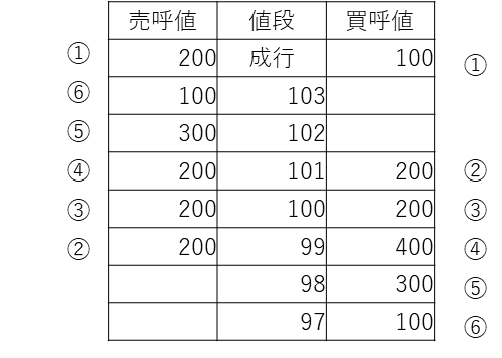
\includegraphics[width=0.49\linewidth]{fig/itayose.pdf}
    \hfil
    \begin{picture}(14,185)
        \put(0,170){(b)}
    \end{picture}
    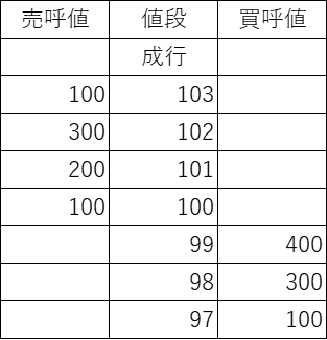
\includegraphics[width=0.335\linewidth]{fig/continuous.pdf}
    \caption{(a) 始値直前の板の状況.(b)始値直後の板の状況.}
    \label{fig:opening}
\end{figure}

\section{市場の性質}
\subsection{確率過程}
確率過程$W = (W_t)_{t \geq 0}$が次の性質1~4を満たすとき,確率過程$W$を標準ブラウン運動,あるいはウィナー過程という\cite{stochastic_integration}.
\begin{enumerate}
    \item $W_0 = 0 \quad a.s.$
    \item 各$0 \leq s \leq t$に対して,$W_t - W_s \sim \mathcal{N}(0, t - s)$
    \item 独立定常増分量である.
    \item 確率1で連続なパスを持つ.
\end{enumerate}

また,ある定数$\mu \in \mathbb{R}, \sigma > 0$とブラウン運動$W_t$を用いて表される確率微分方程式
\begin{equation}
    dS_t = \mu S_t dt + \sigma S_t dW_t \label{eq:geoBrow_equation}
\end{equation}

の解$S_t$は式(\ref{eq:geometric_Brown})で表され,この確率過程$S_t$を幾何ブラウン運動,$\sigma$をボラティリティという\cite{Stochastic_Calculus}.
\begin{equation}
    S_t = S_0 \exp{\left(\sigma W_t + \left( \mu - \frac{1}{2}\sigma^2 \right)t\right)}. \label{eq:geometric_Brown}
\end{equation}

\subsection{ボラティリティ・クラスタリング}
リターン自体は無相関であるが,リターンの絶対値やその2乗はゆるやかに減衰する正の自己相関関数を示す\cite{Cont2007}.
そのため,株価が大きく変化した後は大きな変動が続く傾向があり,小さく変動をした後には小さな変動が続く傾向がある\cite{return_correlation}.
この性質のことをボラティリティ・クラスタリング(volatility clustering)という.

\subsection{ファット・テール}
図(\ref{fig:fat_tail})で示すような,正規分布に比べて裾が厚く,べき乗測に従っている分布に対してファット・テールを持つという表現が用いられる\cite{fat-tailed}.
\begin{figure}[htbp]
    \centering
    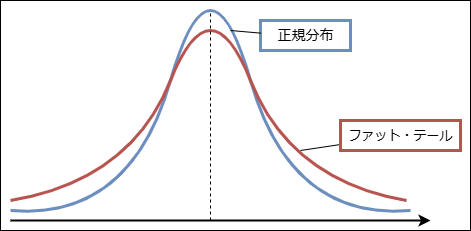
\includegraphics[width=10cm]{fig/fat_tail.png}
    \caption{ファット・テール分布と正規分布}
    \label{fig:fat_tail}
\end{figure}
ファット・テール分布の一種であるパレート分布の確率密度関数は,ある定数$a > 0,b > 0$を用いて式(\ref{eq:power_pdf})で表される\cite{PowerDistribution}.
\begin{equation}
    f(x) = \frac{ab^a}{x^{a + 1}} \qquad (x > b). \label{eq:power_pdf}
\end{equation}
よって相補累積分布関数$P(X \geq x)$は
\begin{equation}
    \begin{aligned}
        P(X \geq x) & = 1 - P(X \leq x)                     \\
                    & = 1 - \int_{b}^{x} f(t) \mathrm{d}t   \\
                    & = \frac{b^a}{x^a} \label{eq:survival}
    \end{aligned}
\end{equation}
となることより,パレート分布の相補累積分布関数は両対数グラフで直線となる.
そのため,ファット・テールを持つ分布の相補累積分布関数は図\ref{fig:fat_tail_survival}のように両対数グラフで一部直線を持つ.

\begin{figure}[htbp]
    \centering
    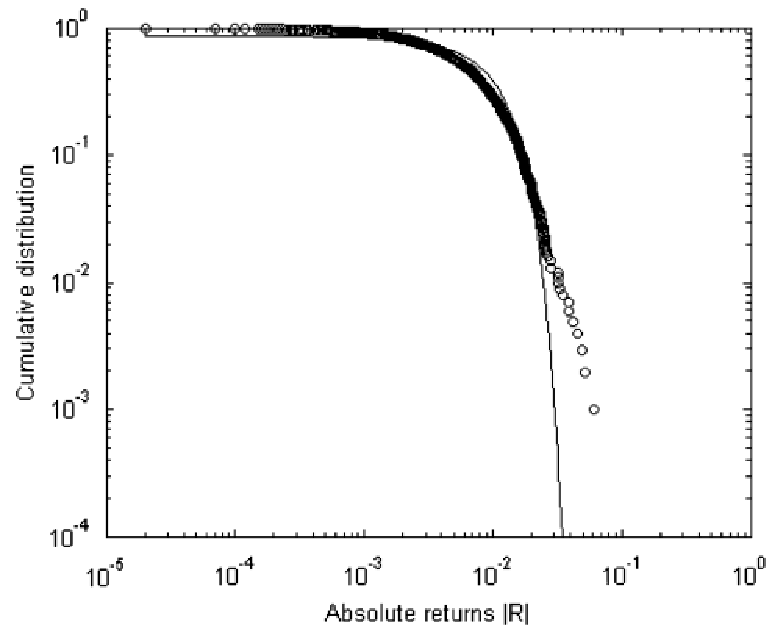
\includegraphics[width=10cm]{fig/fat_tail_survival.pdf}
    \caption{ファット・テールと正規分布の相補累積分布関数\cite{Cont2007}}
    \label{fig:fat_tail_survival}
\end{figure}


\section{Zero-intelligence trader}
Zero-intelligence (ZI) traderは,人間と異なり利益追求や学習を行わず,最低限の制約のみに従ってランダムに取引を行うトレーダーである.\cite{Gode_and_Sunder}

\subsection{GSモデル}
ZI traderの1つにGodeとSunderによって提案されたモデルが存在する\cite{Gode_and_Sunder}.
以降このモデルをGSモデルとする.
GSモデルは,市場規律による予算制約によって行動が制限されること\cite{market_displine}を用いて,ZIトレーダーに予算による制限を設けることで取引価格が均衡価格近傍に収束することや余剰をほぼ最大にするといった市場の特性を再現している.

はじめに各トレーダーには償却価値とコストが与えられ,$i$番目のトレーダーの償却価値を$v_i$,コストを$c_i$とする.
償却価値$v_i$とコスト$c_i$は$[1, V_\mathrm{max}]$の整数の一様乱数に従って生成される.
次に,ランダムなトレーダーを選び確率1/2で売注文を,確率1/2で買注文を出す.
このとき,注文数は1株とし,呼値は売注文の場合は$[c_i, V_\mathrm{max}]$で,買注文の場合は$[1, v_i]$でランダムとする.
ただし,$V_\mathrm{max}$は一株当たりの注文価格の上限とする.
そしてこれまでの注文の記録と比較して,対当できるなら約定を成立させ,対当はできないが記録の中で最も取引が成立しやすい(売注文の場合は安く,買注文の場合は高い)価格である場合は新たにその価格を記録する.
以上の操作を全員が取引を行うか十分に時間が経過するまで繰り返すと,約定価格は図\ref{fig:gode_sunder_trade}の黒線のように変化する.
全トレーダーの呼値を,売注文の場合は昇順に,買注文の場合は昇順に並べることで図\ref{fig:gode_sunder_trade}の赤線と緑線のような需給曲線を引くことができ,約定価格が最終的に均衡価格近傍に収束している.
また,余剰についても需給曲線から求められる最大値の95 \%程度になっている.

予算制約を設けない完全にランダムなトレーダーと人間にも同様の実験を行ったところ完全にランダムなトレーダーのみ取引価格が均衡価格近傍に収束せず,余剰も9割を越えなかった.
そのため,GSモデルによってこれらの市場の特性が市場規律による予算制約によるものだと明らかにされている.
\begin{figure}[htbp]
    \centering
    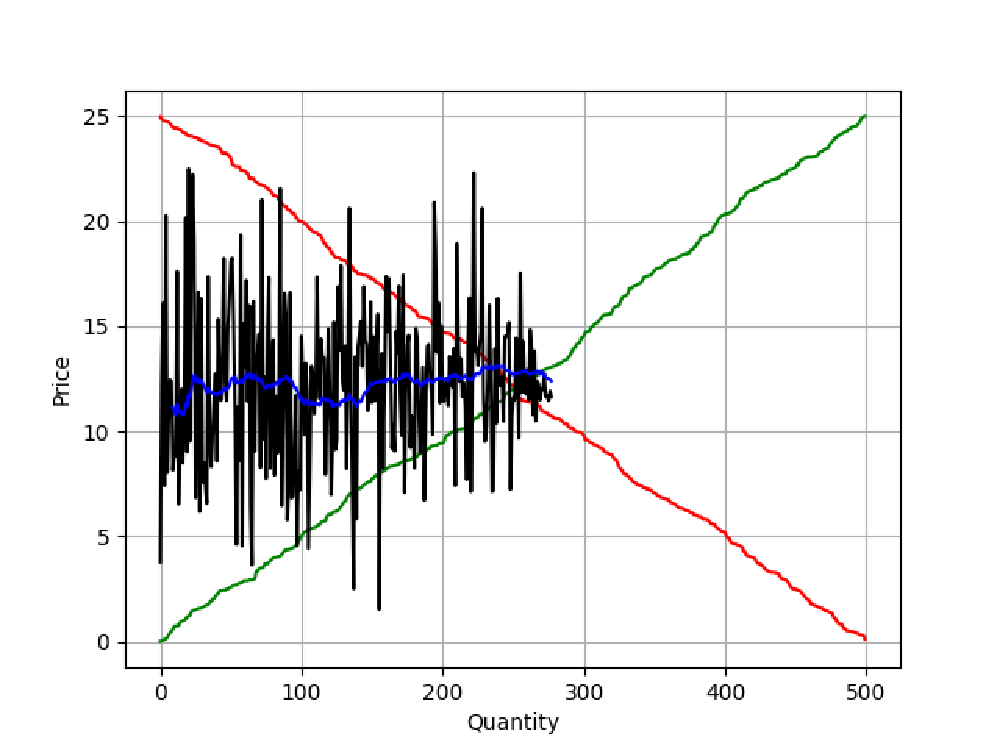
\includegraphics[width=10cm]{fig/gode_sunder_trade.pdf}
    \caption{GSモデルの需給曲線と取引価格.}
    \label{fig:gode_sunder_trade}
\end{figure}


\subsection{Genoaモデル}
GSモデルの他に,トレーダーの注文方法に制限を設け,更にクラスターを形成させることによって,ファット・テールとボラティリティ・クラスタリングを再現したモデルがある\cite{Genoa}.
以降,このモデルをGenoaモデルと呼ぶ.

前提として,トレーダーは限られた資産を用いて単一株を取引する.
また,トレーダーの人数を$N$人として,ステップ$h$における$i$番目のトレーダ-の全資産を$A_i(h)$,現金資産を$C_i(h)$,株価を$p(h)$とする.このとき,ステップ$h + 1$におけるトレーダー$i$の売呼値$s_i(h + 1)$を式(\ref{eq:Genoa_sell}),買呼値$b_i(h + 1)$を式(\ref{eq:Genoa_buy})で決定する.
\begin{equation}
    s_i(h + 1) = \frac{p(h)}{\mathcal{N}(\mu, \sigma_i)}, \label{eq:Genoa_sell}
\end{equation}
\begin{equation}
    b_i(h + 1) = p(h) \mathcal{N}(\mu, \sigma_i). \label{eq:Genoa_buy}
\end{equation}
ただし,$\mathcal{N}(\mu, \sigma_i)$は平均$\mu = 1.01$,標準偏差$\sigma_i$のガウス分布から生成される乱数で,$\sigma_i$は定数$k = 3.5$,時間窓数$T_i = 20$,過去$T_i$間におけるボラティリティ$\sigma(T_i)$を用いて式(\ref{eq:Genoa_sigma_i})で定義される.
\begin{equation}
    \sigma_i = k \sigma(T_i). \label{eq:Genoa_sigma_i}
\end{equation}

また,ステップ$h + 1$におけるトレーダー$i$の売注文の株数$a_i^s$を式(\ref{eq:Genoa_a_i^s}),買注文の株数$b_i^s$を式(\ref{eq:Genoa_a_i^b})に従って決定する.ただし,$r_i$は$[0, 1]$の一様乱数である.
\begin{equation}
    a_i^s = \lfloor r_i A_i(h) \rfloor, \label{eq:Genoa_a_i^s}
\end{equation}
\begin{equation}
    a_i^b = \left\lfloor \frac{r_i C_i(h)}{b_i} \right\rfloor. \label{eq:Genoa_a_i^b}
\end{equation}

GSモデルと同様に全トレーダーの呼値を,売注文の場合は昇順に,買注文の場合は昇順に並べることで需給曲線が得られる.
均衡価格$p^*(h)$は需要曲線と供給曲線の交点として,板寄せと同様の取引方法を用いて,均衡価格$p^*(h)$より安い売呼値と高い買呼値を全て価格$p^*(h)$で売買を成立させる.
そのため
\begin{equation}
    p(h + 1) = p^*(h) \label{eq:Genoa_price}
\end{equation}
となる.
ただし,同じ呼値同士は時間優先の原則ではなく,完全にランダムな優先順位で対当させる.

注文は,基本的には確率1/2で売注文,確率1/2で買注文となるが,クラスターに属している場合は例外が発生する.

各ステップにおいて,すべてのトレーダーのペアについて,確率$P_a$で2人のトレーダー間にクラスターが形成される.
そのため,クラスターはステップが進むにつれて成長や合併を行う.
また,各ステップで確率$P_c$で1つのクラスターをアクティブに,確率$1 - P_c$ですべてのクラスターをインアクティブにする.
アクティブになったクラスターのトレーダーは,全員の出す注文の種類(売注文か買注文か)が同じになり,取引後にクラスターを消滅させる.

\section{Binder cumulant}
相転移や臨界現象の分野ではBinder cumulantと呼ばれる値が重要な役割を果たす\cite{Binder_cumulant}.
Binder cumulnatは式(\ref{eq:Binder})によって定義され, 正規乱数の場合は$U = 0$となる.
そのため,本研究においてはBinder cumulantが0に近い値をとるかを,分布が正規分布であるかを見分ける指標として用いる.

\begin{equation}
    U = 1 - \frac{\langle m^4 \rangle}{(\langle m^2 \rangle)^2}. \label{eq:Binder}
\end{equation}


\chapter{手法} \label{chap:method}
\section{GSモデルの解析}
本研究では,はじめにGSモデルのトレーダーの資産が幾何ブラウン運動に従っているか,LeBaronらによって作成されたGSモデルのコード\cite{Gode_and_Sunder_code}をもとに解析をおこなった.

\subsection{GSモデルの設定}
LeBaronらのコードでは取引期間が1期間のみであったため,取引期間$T$を新たに追加して,複数期間にわたって取引が行うことができるように変更した.
また,トレーダーが1期間に売注文と買い注文を1回ずつの最大2回取引を行うことができたので,売注文か買注文のいずれかを最大1回のみ出すことができるように変更をおこなった.
更に,各トレーダーに資産の項目を追加した.
トレーダーの人数を$N$人として,期間$h$における$i$番目のトレーダーの資産を$A_i(h)$,取引価格を$p(h)$で表し,売注文が成立した場合は式(\ref{eq:Gode_asset_sell}),買い注文が成立した場合は式(\ref{eq:Gode_asset_buy})のように資産を変動させた.
\begin{equation}
    A_i(h + 1) = A_i(h) + p(h), \label{eq:Gode_asset_sell}
\end{equation}
\begin{equation}
    A_i(h + 1) = A_i(h) - p(h). \label{eq:Gode_asset_buy}
\end{equation}
このとき,$A_i(h + 1)$が負の値をとることを許した.

シミュレーションに用いたパラメータを表\ref{tbl:Gode_param}に示す.

\begin{table}[htbp]
    \begin{center}
        \caption{GSモデルの解析で用いたパラメータ}
        \begin{tabular}{lr}
            \hline\hline
            トレーダーの人数 $N$          & 2000 \\
            期間 $T$                      & 100  \\
            呼値の上限 $V_\mathrm{max} $  & 25   \\
            トレーダーの初期資産 $A_i(0)$ & 500  \\ \hline
            \label{tbl:Gode_param}
        \end{tabular}
    \end{center}
\end{table}

以上のシミュレーションを,それぞれの期間において償却価値$v_i$とコスト$c_i$を変化させる場合と変化させない場合について資産分布と資産変動の解析をおこなった.

\subsection{GSモデルの解析方法}
トレーダーの資産分布と資産変動がファット・テールになっているか,相補累積分布関数を作成して標準正規乱数の相補累積分布関数と比較した.

資産分布は,まずトレーダーの最終的な資産$A_1(T), A_2(T), ..., A_N(T)$について平均$\mu_A$と標準偏差$\sigma_A$を求め,式(\ref{eq:normalization})に従って標準化された資産$\tilde{A_1}, \tilde{A_2}, ..., \tilde{A_N}$を得た.
\begin{equation}
    \tilde{A_i} = \frac{A_i(h) - \mu_A}{\sigma_A}. \label{eq:normalization}
\end{equation}
次に,$N$個の標準正規乱数$Z_1, Z_2, ..., Z_n$を用意し,$\tilde{A_1}, \tilde{A_2}, ..., \tilde{A_N}$と$Z_1, Z_2, ..., Z_n$に対して絶対値をとり,それぞれの相補累積分布関数の両対数グラフの比較をおこなった.

資産変動は,トレーダー$i$の資産$A_i(1), A_i(2), ...A_i(T)$について,取引を行われていない,つまり$A_i(h) = A_i(h + 1)$の場合は$A_i(h + 1)$を除外した新たな資産変動のリスト$A_i'(1), A_i'(2), ...A_i'(T')$を作成した.
次に式(\ref{eq:asset_return})に従って資産の変動の割合$R_i(1), R_i(2), ..., R_i(T' - 1)$を求め,資産$A_1(T), A_2(T), ..., A_N(T)$と同様の手順で標準正規乱数との相補累積分布関数の両対数グラフの比較をおこなった.
ただし,$T = 100$とし,各期間ごとにトレーダーの予算制約を変更した.
\begin{equation}
    R_i(h) = \frac{A_i(h)-A_i(h - 1)}{A_i(h - 1)}. \label{eq:asset_return}
\end{equation}

次に,予算制約を変更することによって取引にどのような影響を及ぼすのか調べるために,100期間における分散の時間変化を,予算制約を変更する場合としない場合で比較した.

\section{Genoaモデルの導入}
GSモデルの資産変動の分布がファット・テールを持つようにするために,Genoaモデルを参考に注文数や取引方法に変更を加える.

\subsection{GSモデルから変更しない点}
GSモデル同様,各トレーダーには償却価値$v$とコスト$c$が与えた.
ただし,償却価値とコストは各期間ごとに与えられ,呼値の最大値を$V_\mathrm{max}$とすると,期間$h$のトレーダー$i$の償却価値$v_i(h)$とコスト$c_i(h)$は式(\ref{eq:model_value}),(\ref{eq:model_cost})によって求められる.
ここで,$r_i$,$r_i'$は$[0, 1]$の一様乱数とする.
\begin{equation}
    v_i(h) = \lfloor r_i V_\mathrm{max} \rfloor, \label{eq:model_value}
\end{equation}
\begin{equation}
    c_i(h) = \lfloor r_i' V_\mathrm{max} \rfloor. \label{eq:model_cost}
\end{equation}
トレーダー$i$の期間$h$における売呼値$s_i(h)$は式(\ref{eq:model_sell})で,買呼値$b_i(h)$は式(\ref{eq:model_buy})で決定した.
ただし,$r_i$,$r_i'$は$[0, 1]$は式(\ref{eq:model_value}),(\ref{eq:model_cost})とは異なる値とする.
\begin{equation}
    s_i(h) = \lceil c_i + r_i' (V_\mathrm{max} - c_i), \rceil \label{eq:model_sell}
\end{equation}
\begin{equation}
    b_i(h) = \lfloor v_i - r_i (v_i - 1) \rfloor. \label{eq:model_buy}
\end{equation}

また,トレーダーは確率1/2で,売注文を確率1/2で買注文を出す.

\subsection{GSモデルからの変更点}
トレーダーが複数株注文できるようにするために,取引をGenoaモデルと同様の手順で取引をおこなうように変更した.
具体的には,均衡価格$p^*(h)$より安い売呼値と高い買呼値を全て価格$p^*(h)$で売買を成立させ,同じ呼値同士は完全にランダムな優先順位で対当させた.
そのため,式(\ref{eq:Genoa_price})が成り立つ.

また,Genoaモデルの式(\ref{eq:Genoa_a_i^s}),(\ref{eq:Genoa_a_i^b})を参考に,複数株注文するように変更をおこなった.
トレーダーに保有株数の項目を追加し,期間$h$におけるトレーダー$i$の総資産$A_i(h)$を,保有株数$S_i(h)$と現金資産$C_i(h)$を用いて式(\ref{eq:model_asset})のように定義する.
\begin{equation}
    A_i(h) = p(h) S_i(h) + C_i(h). \label{eq:model_asset}
\end{equation}
総資産$A_i$と現金資産$C_i$を用いて,ステップ$h$におけるトレーダー$i$の売注文数$n_i^s(h)$を式(\ref{eq:model_num_sell})に,買注文数$n_i^b(h)$を式(\ref{eq:model_num_buy})に従って決定した.ただし,$r_i$,$r_i'$は$[0, 1]$の一様乱数,$\alpha, \beta$は$[0, 1]$の定数とし,資産の何倍を使って注文するかを表す.
\begin{equation}
    n_i^s(h) = \frac{r_i \alpha A_i(h)}{p(h)}, \label{eq:model_num_sell}
\end{equation}
\begin{equation}
    n_i^b(h) = \frac{r_i' \beta C_i(h)}{p(h)}. \label{eq:model_num_buy}
\end{equation}

$\alpha$を$0.03, 0.06, 0.09, 0.12, 0.15, 0.18, 0.21, 0.24, 0.27$,$\beta$を$0.05, 0.1, 0.2, 0.3, 0.4, 0.5, 0.6, 0.7, 0.8, 0.9$と変化させて取引をおこない,資産変動とリターンの相補累積分布関数の図がどのように変化するのか調べた.

式(\ref{eq:over_oder})のように注文価格の合計や注文株数が保有している量を上回る場合は,可能な限り取引をおこなうように,$n_i^s(h)$と$n_i^b(h)$を式(\ref{eq:changed_num_order})に変更した.
\begin{equation}
    S(h) < n_i^s(h), \quad C(h) < b_i(h) n_i^b(h), \label{eq:over_oder}
\end{equation}
\begin{equation}
    n_i^s(h) = S(h), \quad n_i^b(h) = \left \lfloor \frac{C(h)}{b_i(h)} \right \rfloor. \label{eq:changed_num_order}
\end{equation}




\chapter{結果} \label{chap:results}
\section{GSモデルの特性}\label{chap:result_GS}
\subsection{GSモデルの従う確率過程}
トレーダーの資産変動の相補累積分布関数を図\ref{fig:GS_survivalD}(a)に,資産分布の相補累積分布関数を図\ref{fig:GS_survivalD}(b)に,リターンの相補累積分布関数を図\ref{fig:GS_survivalD}(c)に示す.
図\ref{fig:GS_survivalD}(a)より,トレーダーの資産変動の分布はファット・テールを持たず,図\ref{fig:GS_survivalD}(b)よりトレーダーの資産分布は指数分布になっていることが確認された.
そのため,GSモデルのトレーダーの資産は標準ブラウン運動に従っており,幾何ブラウン運動には従っていなかった.
同様にリターンの分布についてもファット・テールを持っておらず,市場規律は資産やリターンがファット・テール分布になる要因でないことが分かった.
\begin{figure}[htbp]
    \centering
    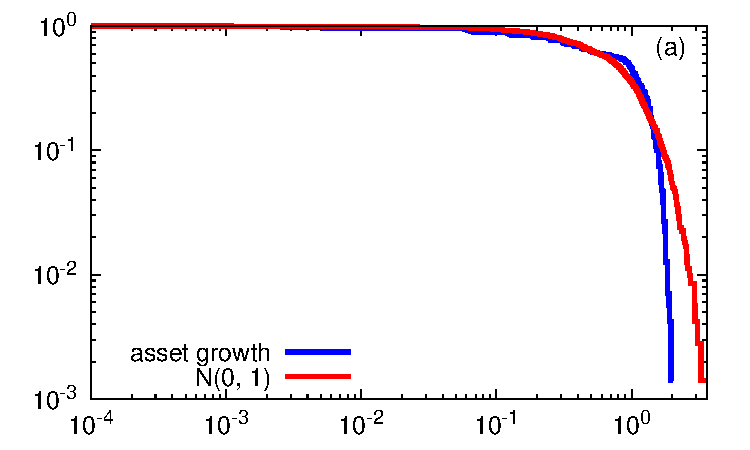
\includegraphics[width=10cm]{fig/Brown/asset_growth_brown.pdf}
    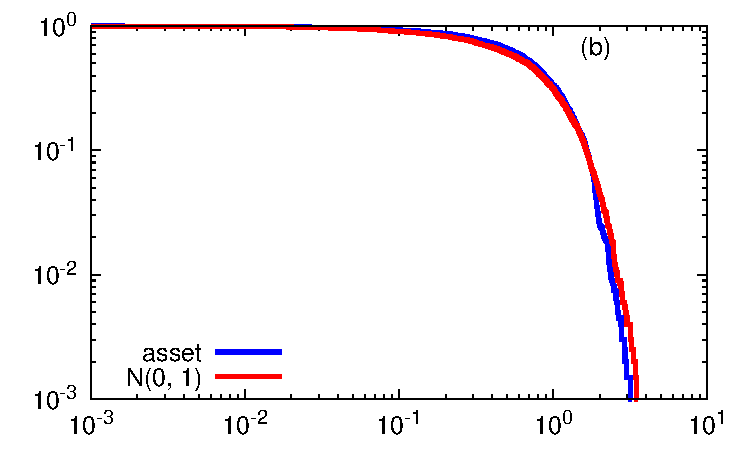
\includegraphics[width=10cm]{fig/Brown/asset_brown.pdf}
    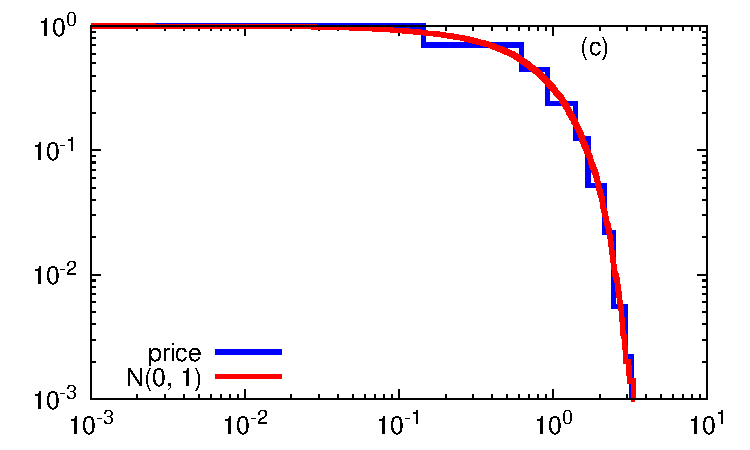
\includegraphics[width=10cm]{fig/Brown/price_brown.pdf}
    \caption{GSモデルのトレーダーの(a)資産変動と(b)資産と(c)リターンの相補累積分布関数}
    \label{fig:GS_survivalD}
\end{figure}

\subsection{予算制約と資産の分散の関係}
GSモデルについて,償却価値などの予算制約を期間ごとに変更した場合のトレーダーの資産の分散の時間変化を図\ref{fig:GS_variance}(a)に,価格戦略を固定した場合の分散の時間変化を図\ref{fig:GS_variance}(b)に示す.
予算制約を変更した場合は,グラフが直線的になっていることより分散は時間$t$に比例しており,diffusiveになっている.
一方で価格戦略を固定した場合は,分散は$t^2$に比例し,ballisticになっている.
\begin{figure}[htbp]
    \centering
    \begin{picture}(14,130)
        \put(4,230){(a)}
    \end{picture}
    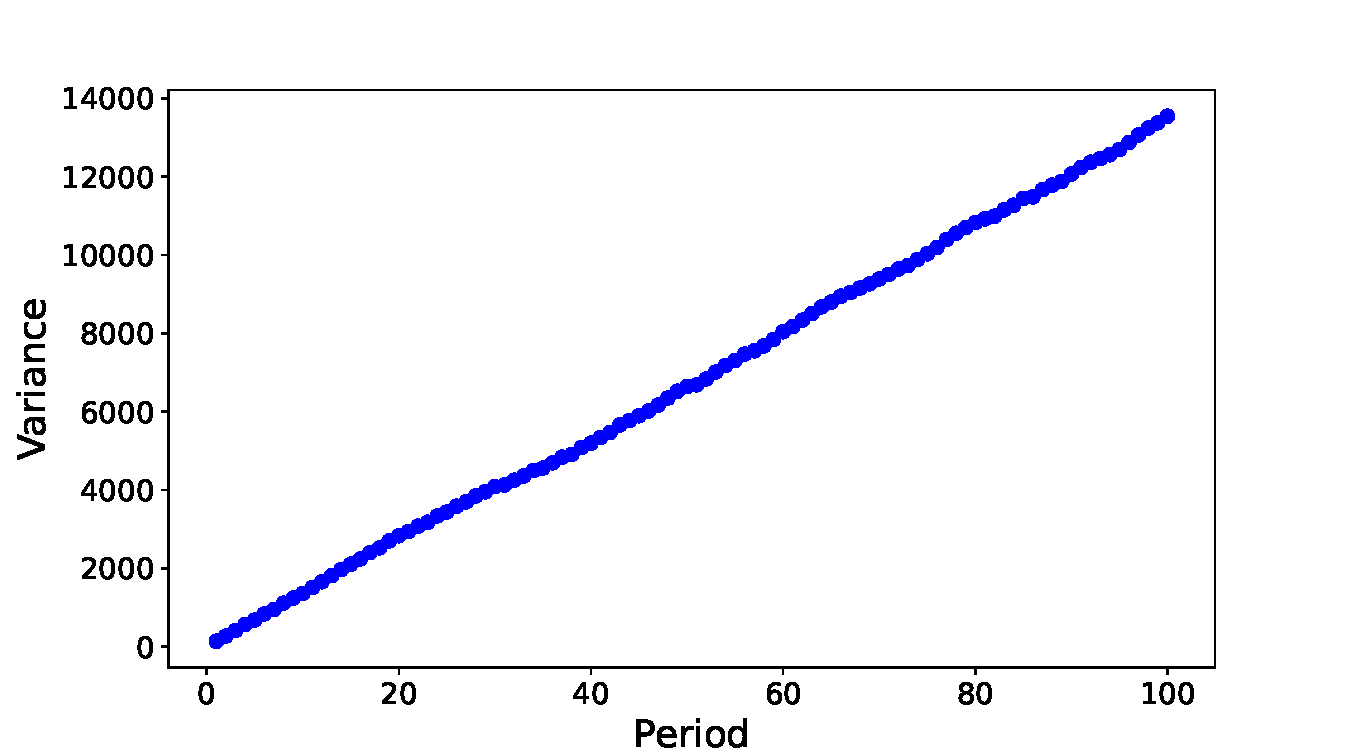
\includegraphics[width=0.95\linewidth]{fig/Var.pdf}
    \begin{picture}(14,130)
        \put(4,230){(b)}
    \end{picture}
    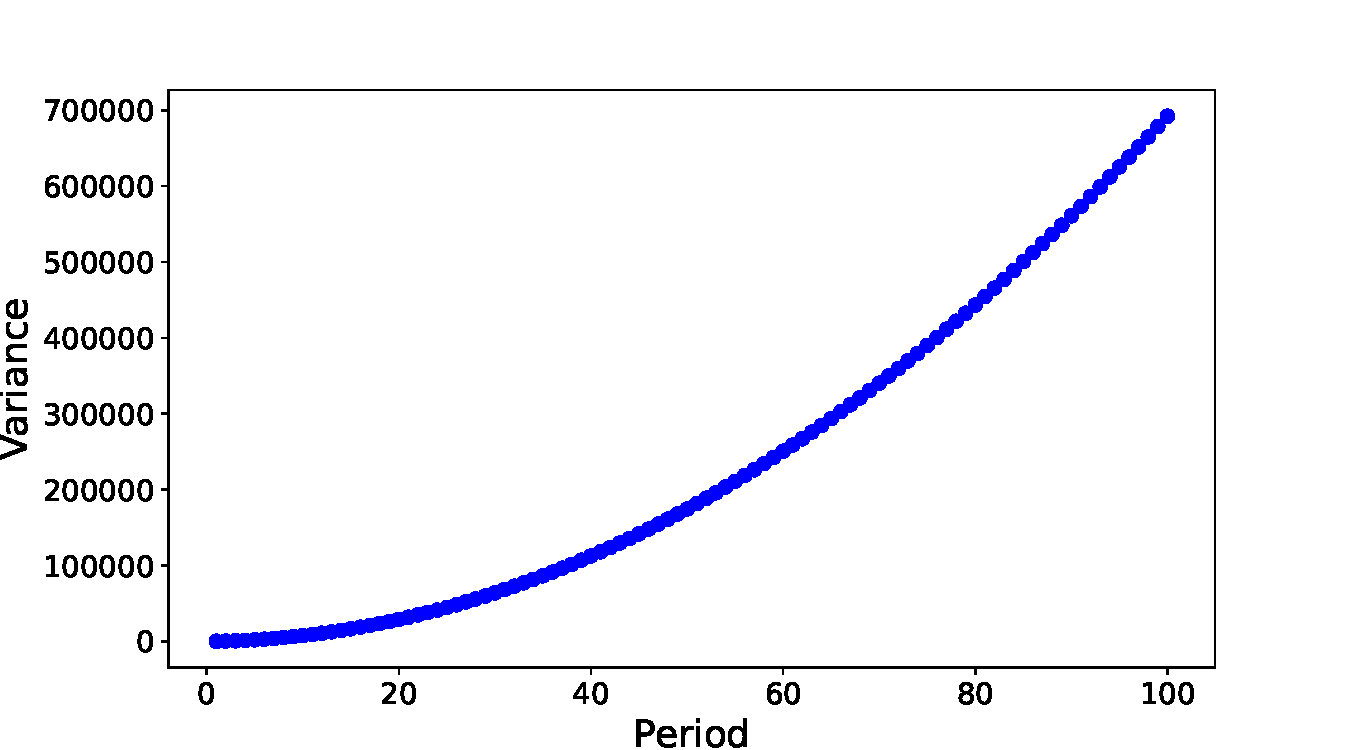
\includegraphics[width=0.95\linewidth]{fig/Var2.pdf}
    \caption{(a)予算制約を変更した場合の分散の時間変化, (b)予算制約を固定した場合の分散の時間変化}
    \label{fig:GS_variance}
\end{figure}


\section{モデル拡張後の各分布}\label{chap:model}
\subsection{リターンの分布}\label{chap:model_return}
リターンの相補累積分布関数の両対数グラフを図\ref{fig:model_return}に示す.
リターンの分布はガウス分布と一致しており,ファット・テール分布になっていないことが読み取れる.
そのため,トレーダが自身の資産に比例して注文を出すことは,リターンがファット・テール分布になる要因ではないことが分かった.

\begin{figure}
    \centering
    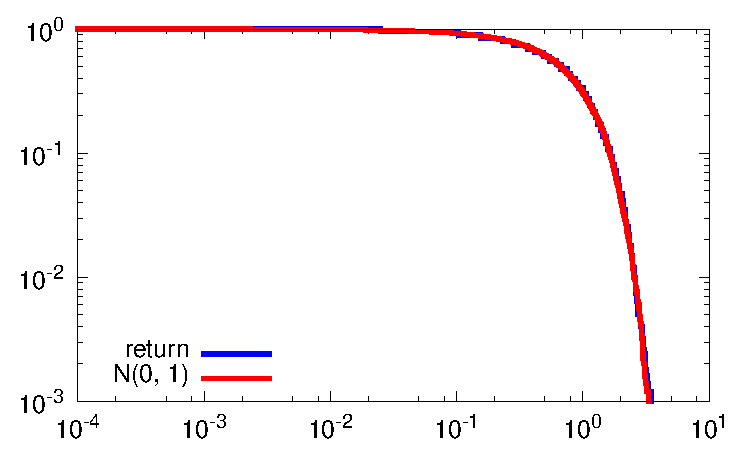
\includegraphics[width=10cm]{fig/return_survival.pdf}
    \caption{リターンの相補累積分布関数.}
    \label{fig:model_return}
\end{figure}

\subsection{資産の分布と資産変動の分布}\label{chap:model_asset}
資産の相補累積分布関数の例を図\ref{fig:model_asset_survival}に示す.
分布は,図\ref{fig:model_asset_survival}(a)のようにファット・テール分布になる場合と,(b)のように正規分布になる場合と,(c)のように段々になる場合の3種類に分かれた.

\begin{figure}[htbp]
    \centering
    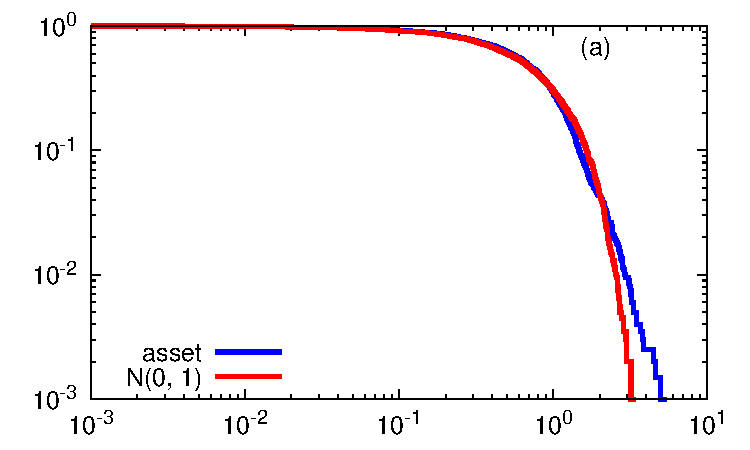
\includegraphics[width=0.7\linewidth]{fig/asset_a012_b02.pdf}
    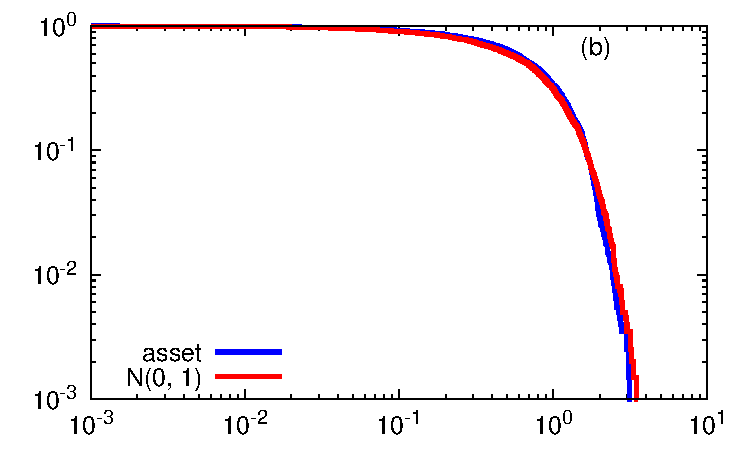
\includegraphics[width=0.7\linewidth]{fig/asset_a003_b01.pdf}
    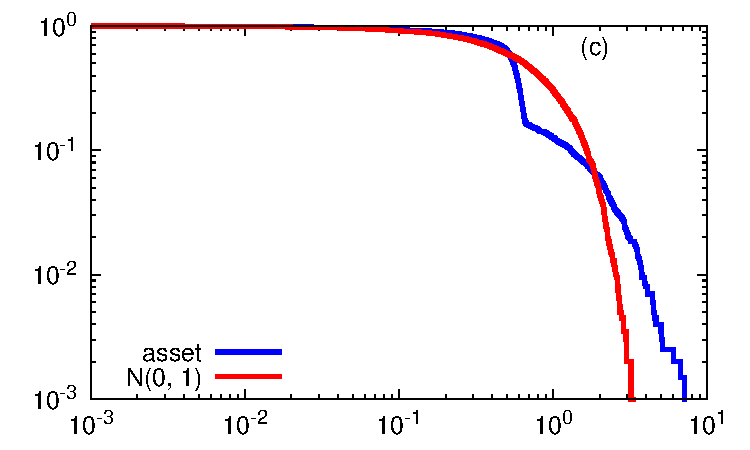
\includegraphics[width=0.7\linewidth]{fig/asset_a05_b05.pdf}
    \caption{資産の相補累積分布関数(a)$\aleph = 0.12, \beta = 0.2$, (b)$\aleph = 0.03, \beta = 0.1$,(c)$\aleph = 0.5, \beta = 0.5$.}
    \label{fig:model_asset_survival}
\end{figure}

資産変動の相補累積分布関数の例を図\ref{fig:model_asset_growth_survival}に示す.
資産変動についても資産分布同様,3種類の分布に分かれた.

\begin{figure}[htbp]
    \centering
    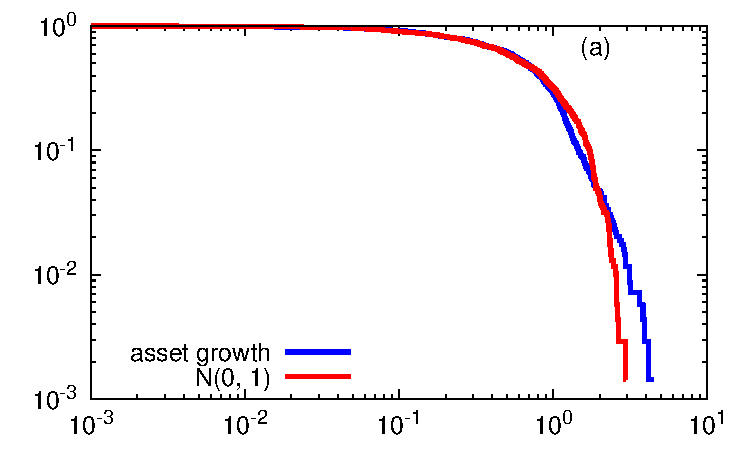
\includegraphics[width=0.7\linewidth]{fig/asset_growth_a015_b03.pdf}
    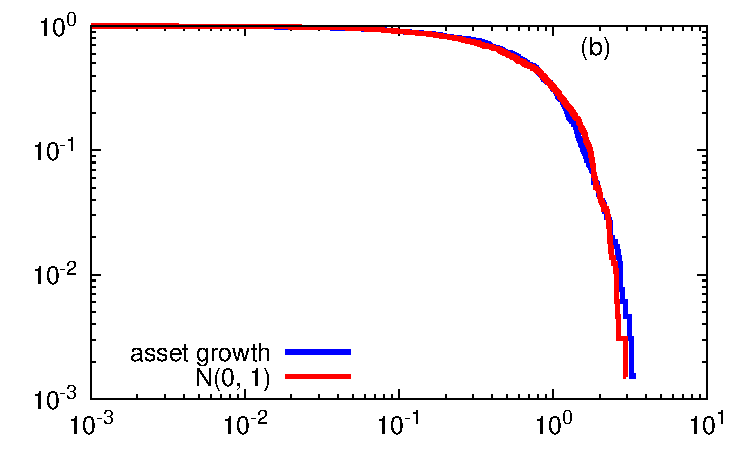
\includegraphics[width=0.7\linewidth]{fig/asset_growth_a003_b02.pdf}
    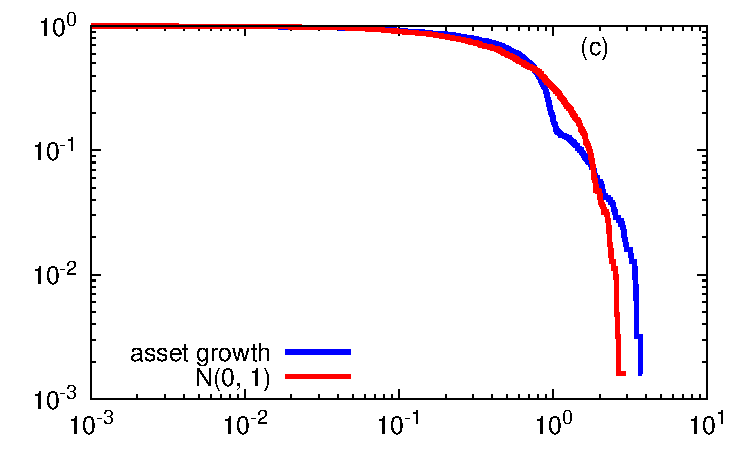
\includegraphics[width=0.7\linewidth]{fig/asset_growth_a05_b05.pdf}
    \caption{資産変動の相補累積分布関数(a)$\aleph = 0.15, \beta = 0.3$, (b)$\aleph = 0.03, \beta = 0.2$,(c)$\aleph = 0.5, \beta = 0.5$.}
    \label{fig:model_asset_growth_survival}
\end{figure}


各$\alpha, \beta$における分布の種類の相図を,資産分布は図\ref{fig:signal_asset}に,資産変動は図\ref{fig:signal_asset_growth}に示す.
図より,ファット・テール分布が現れやすい$\alpha, \beta$の範囲が存在し,資産分布の場合は$\alpha$が0.27以下,$\beta$が0.4以下,資産変動の場合は$\alpha$が0.06~0.27,$\beta$が0.2~0.5と読み取れる.
また,いずれにおいても$\alpha$が0.3を超えると,$\beta$の値に関わらず,図\ref{fig:signal_asset}(c)で示すような非単調な振る舞いをとることが分かった.


\begin{figure}
    \centering
    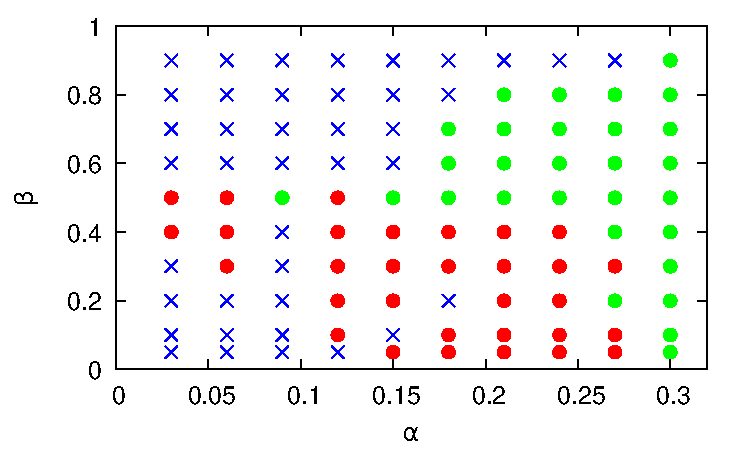
\includegraphics[width=0.9\linewidth]{fig/signal.pdf}
    \caption{資産分布の相図}
    \label{fig:signal_asset}
\end{figure}

\begin{figure}
    \centering
    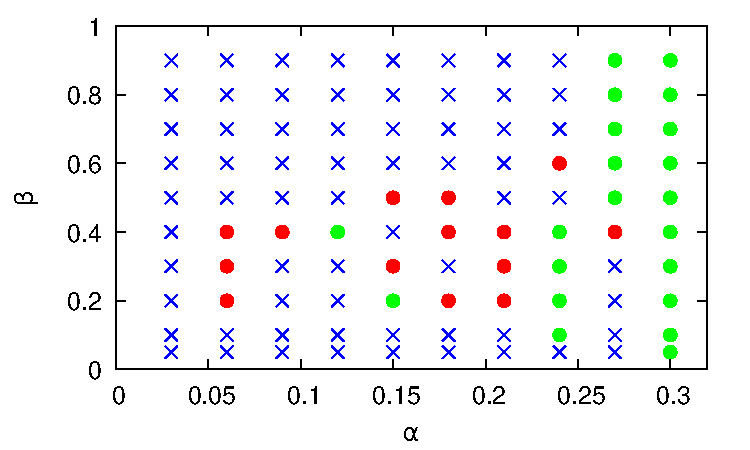
\includegraphics[width=0.9\linewidth]{fig/signal/signal_asset_growth.pdf}
    \caption{資産変動の相図}
    \label{fig:signal_asset_growth}
\end{figure}


\chapter{考察および結論} \label{chap:summary}
\section{考察}
\subsection{Genoaモデルの特性の要因}
\ref{chap:model}節の結果より,トレーダーが自身の資産に比例して注文を出す制約は,リターンがファット・テール分布になる直接的な要因ではないが資産分布や資産変動がファット・テール分布になる要因であることが分かった.
そのため,リターンがファット・テール分布になる要因は,注文価格を,ボラティリティを変数に持つ正規乱数と株間の関数に従って決定していること,もしくはクラスターの形成方法のどちらかであると考えられる.

\subsection{分布における非単調な振る舞い}\label{chap:step}
\ref{chap:model_asset}節において図\ref{fig:model_asset_survival}(c)の分布のような,正規分布やファット・テール分布とは異なり、変曲点を複数持つような分布が得られた.
この原因として,トレーダーが資産のほとんどを用いて取引を行うことにより,資産分布に偏りが生じていることが原因であると考えられる.
実際$\alpha = 0.5, \beta = 0.5$におけるトレーダーの資産分布は図\ref{fig:hist_asset}のようになり,パレート分布と比較してもトレーダーの資産分布は偏っている.
また,注文は資産に比例して出されるため,資産分布が偏っているとき,資産変動も偏った値をとると考えられる.
非常に小さな値の資産や資産変動が大量に発生することにより,段のような分布が形成されると考えられる.

\begin{figure}
    \centering
    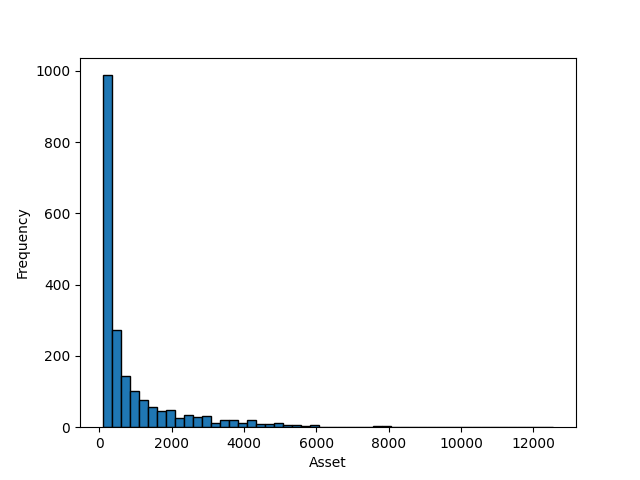
\includegraphics[width=10cm]{fig/hist.png}
    \caption{$\alpha = 0.5, \beta = 0.5$における資産分布}
    \label{fig:hist_asset}
\end{figure}


\subsection{売り制約と買い制約の変数依存性の違い}
図\ref{fig:signal_asset}, \ref{fig:signal_asset_growth}においてファット・テール分布が現れる範囲の値が$\alpha$と比較して$\beta$の方が大きい.
式(\ref{eq:model_asset})-(\ref{eq:model_num_buy})から,買注文の場合は現金資産$C_i(h)$に比例して注文をおこなうが,売注文では現金資産$C_i(h)$にリスク資産$S_i(h)$を加えた,総資産$A_i(h)$に比例して注文をおこなう.
そのため,$\alpha$と$\beta$が等しい値の場合,売注文の方が注文数が多くなりやすく,図\ref{fig:hist_asset}のような分布になりやすく,相補累積分布関数がファット・テール分布ではなく,非単調な分布になりやすいと考えられる.
これは,図\ref{fig:signal_asset}, \ref{fig:signal_asset_growth}において,段々になっている分布が$\beta$のみの値が大きい場合は現れないが,$\alpha$の値が大きくなると$\beta$の値に関わらず現れるため,\ref{chap:step}節の考えと一致する.

\section{結論と今後の展望}
本研究ではGSモデルが幾何ブラウン運動に従っておらず,資産分布と資産変動がガウス分布になっていることを確認し,Genoaモデルの制約の一部を課すことで,ファット・テール分布が現れる条件を調査した.
その結果,売注文と買注文の上限によってトレーダーの資産分布は変化し,ファット・テール分布を含め,三種類の分布が現れた.
また,Genoaモデルのトレーダーの資産に比例した株数を注文するという制約は,リターンがファット・テール分布になる要因ではないが,資産分布や資産変動がファット・テール分布になる要因であることが判明した.

今後の展望として,現状トレーダーは単一種類の株しか取引をおこなえないので,複数種類の株を取引できるように拡張し,複数資産に投資することでボラティリティが減少するのかの検証をおこないたい.

\chapter*{謝辞}
はじめに指導教員である渡辺宙志先生にお礼申し上げます.
金融という物理情報工学科に関連のない分野にもかかわらず,研究の方向性や方法など様々な助言を送っていただいたことや,プログラミングやソフトウェアの知識に疎い私に対して丁寧に指導していただいたことなど,これらの貴重なアドバイスや指導が私の研究や成長に大いに役に立ちました.


また,研究室ミーティングや練習発表会で質問や助言を与えてくださった先輩方にも感謝しております.
特に,研究室でお会いする機会の多かった小林さんと竹内さんからは,研究への取り組み方だけでなく,自身が関心を抱く分野への取り組み方について,多くのことを学ばせていただきました.

そして,研究室の同期の皆さんにも感謝しております.
中でも伊藤君は機械の操作方法やハンズオンの内容が理解できていなかった私に対して,その都度アドバイスをくれました.
現在,私が問題なく研究を継続できているのは,伊藤君のおかげです.

最後に,これまで私を支えてくれた両親に心よりお礼申し上げます.
本研究に取り組むことができたのは,大学進学や日常生活において自由な選択肢を与え、それらを支えてくれた両親のおかげです.
ありがとうございました.

\appendix

\chapter{ソースコード}

\lstinputlisting[caption = Gode and Sunderモデルのダブルオークションシミュレーションコード, label = prog:script]{src/script.py}
\lstinputlisting[caption =トレーダーの注文に関するコード, label = prog:agent]{src/agent.py}
\lstinputlisting[caption = 取引をおこない,株価を決定するコード, label = prog:openPrice]{src/openPrice.py}
\lstinputlisting[caption = グラフとデータを作成するコード, label = prog:survivalFunction]{src/survivalFunction.py}
\lstinputlisting[caption = yamlファイルとpltファイルを作成するコード, label = prog:makeseed]{src/makeseed.py}

\bibliographystyle{junsrt}
\bibliography{reference}

\end{document}
